\chapter{State of the Art}
\label{chap:soa}

\section{The Artificial Intelligence Spectrum}
%%Referencias a los tipos de modelos y a los modelos hibridos que hay y a los estudios quasifilosoficos sobre por que unos pisan a otros, reemplazan a otros, mejoran a otros, etc.

\begin{figure*}
    \centering
    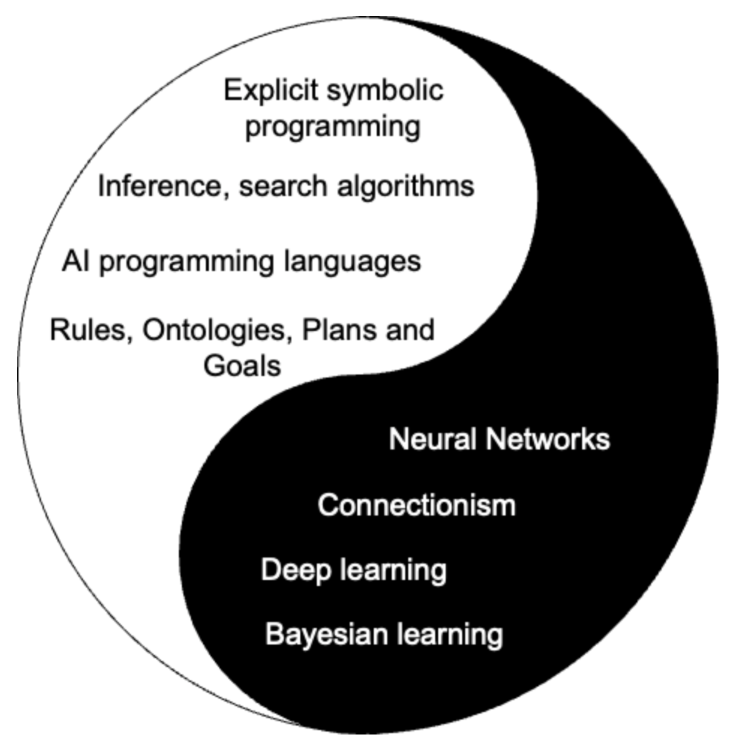
\includegraphics[width=.5\linewidth]{3_stateoftheart/figures/Lieberman_taxonomy.eps}
    \caption{AI Spectrum as depicted in \cite{lieberman_symbolic_nodate}}
    \label{fig:lieberman_tax}
\end{figure*}

Throughout the years, several categorizations have been proposed for the existing Artificial Intelligence (AI) models, each attending to a specific criteria. \cite{lieberman_symbolic_nodate} categorizes AI models considering their input in two categories: symbolic (also referred to as "classic AI") and subsymbolic. These two types are disjoint and complimentary to each other. \cite{lieberman_symbolic_nodate} depicts the AI spectrum as a \textit{yin-yang} (Figure \ref{fig:lieberman_tax}), where the flaws of one kind are compensated by the benefits of the other. While this categorization presents a simple and general overview on the existing AI models, it lacks a middle ground where hybrid approaches can be categorized. 

Opposite to this vision, where the focus is on the input, \cite{loyola-gonzalez_black-box_2019} envisions the AI spectrum from the perspective of the output. This taxonomy categorizes AI approaches as \textit{white-box} or \textit{black-box} considering whether the process that lead to a given output can be explained or not. The notation \textit{black-box} is used to describe those models whose inference process cannot be explain, which mainly applies to machine learning models.  \textit{Black-box} models can be subsequently grouped in: hyperplane-based (Support Vector Machines), neural networks (Convolutional Neural Networks, Graph Neural Networks), probability-based (Probabilistic Logic Networks) and instance-based (K-nearest neighbours). On the opposite side of this spectrum lie \textit{white-box} models, which relate to those approaches whose inference process can be understood and explain. Decision trees, rule-based systems or fuzzy logic are encompassed in this category.


\begin{figure}
    \centering
    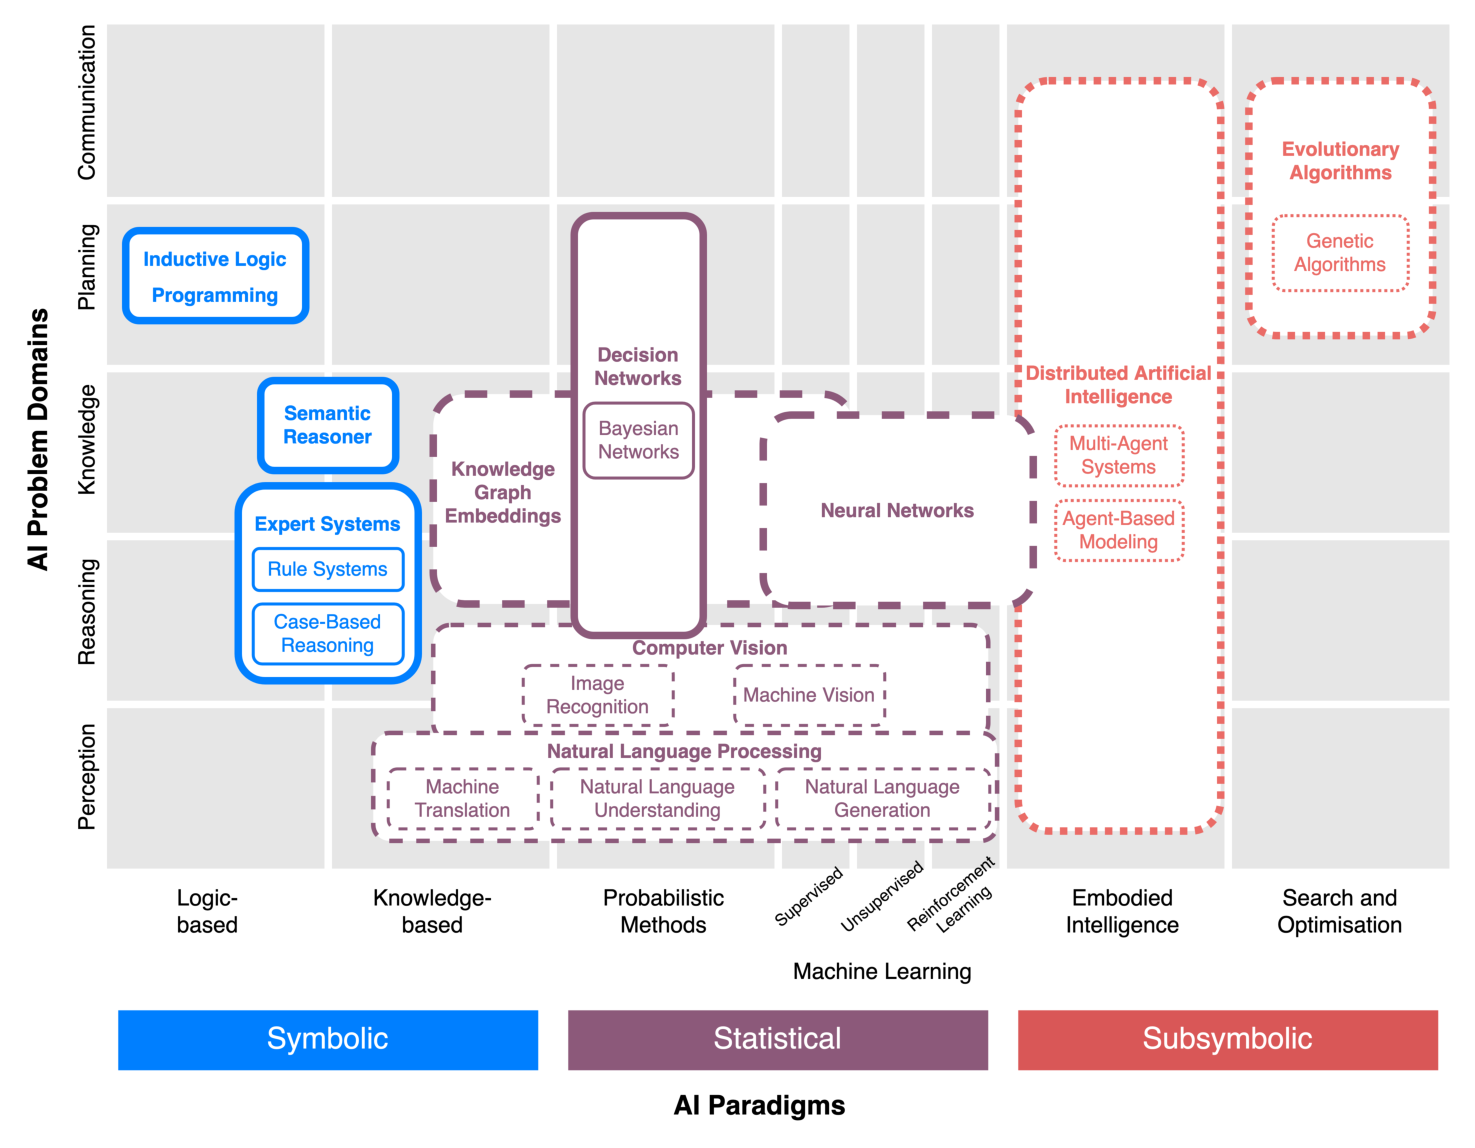
\includegraphics[width=\linewidth]{3_stateoftheart/figures/AI_Map.eps}
    \caption{Map of AI models combining the taxonomy of \cite{corea_ai_2019} with the taxonomy considered in this thesis. Symbolic, statistical and subsymbolic approaches are colour-coded in blue, purpe and red respectively. Knowledge-based and computational intelligent systems are coded in continuous and non-continuous lines, respectively. Dashed lines depict deep learning approaches, while dotted lines depict other computational intelligent approaches.}
    \label{fig:ai_map}
\end{figure}


More recently, \cite{corea_ai_2019} proposed a two dimensional categorization of AI technologies. Instead of considering the input or output of the model, this taxonomy focuses on the application domains of each paradigm and its reasoning paradigm. Figure \ref{fig:ai_map} portrays this categorization, where the Y-Axis comprises the existing problem domains, while the X-Axis encodes the three considered paradigms: symbolic, statistical and subsymbolic. While the taxonomy proposed by \cite{lieberman_symbolic_nodate} only considered the symbolic (blue) and subsymbolic (red) categories, \cite{corea_ai_2019} also considers the statistical (purple) models, as an in-between group between the two complimentary groups. Moreover, finer-grained subcategories can be distinguished inside each of the three main paradigms:
\begin{itemize}
    \item \textbf{Symbolic models:} As previously described, the term \textit{symbolic} describes AI paradigms that not only employ symbolic representations as input, but have an inference process that can be understood and explained by humans. Two finer grained types are identified inside this category: logic-based and knowledge-based.
    \item \textbf{Statistical models:} While the taxonomy proposed by \cite{lieberman_symbolic_nodate} only comprised symbolic and subsymbolic models, which are treated as analogous and complimentary kinds, this taxonomy distinguishes statistical models from purely subsymbolic models. These models employ mathematical tools for reasoning, and can be subsequently divided into probabilistic and machine lerning models.
    \item\textbf{Subsymbolic models:} According to this taxonomy, the term \textit{symbolic} refers to the absence of previous knowledge needed to function. Embodied intelligence models and search and optimisation models are grouped under this criterion.
\end{itemize}

The previous taxonomies provided categories that were fully disjoint and, therefore, each particular model needed to belong to exclusively one of the types. The taxonomy of \cite{corea_ai_2019} enables a higher degree of flexibility, as models can be applied under different problem domains as well as use different reasoning paradigms.
%%Taxonomias de la mas antigua a la mas moderna
\cite{hopgood_2009_knowledge-based} proposed a division of AI paradigms in two main categories: knowledge-based systems and computationally intelligent systems. Knowledge-based systems require explicit representations of knowledge in a symbolic form, while computationally intelligent systems use nature-inspired paradigms where no background knowledge is required to reason. This taxonomy can be merged with the taxonomy of \cite{corea_ai_2019}, providing a three-dimensional taxonomy as depicted in Figure \ref{fig:ai_map}. A third dimension depicting whether the paradigm can be classified as knowledge-based (continuous line) or computationally intelligent (discontinuous line). 

Deep Learning was introduced after \cite{hopgood_2009_knowledge-based} taxonomy was defined and, therefore, it did not cover these models. Therefore, a slight update on this base taxonomy is proposed to include deep learning models. Figure \ref{fig:ai_map} makes a distinction inside the computationally intelligent models, denoting in a dashed instead of a dotted line those paradigms that can be considered as deep learning. 

After combining the taxonomies presented in \cite{hopgood_2009_knowledge-based} and \cite{corea_ai_2019}, the final categorization of models is as follows:
\begin{itemize}
    \item \textbf{Knowledge-Based Systems:} These system fit almost perfectly the definition previously provided for the symbolic paradigms. Therefore, this category groups all the models that require from background expert knowledge to reason:
    \begin{itemize}
        \item \textit{Inductive Logic Programming (ILP):} This term was first introduced by \cite{Muggleton1991}, describing this field as "\textit{the area of AI which deals with the induction of hypothesised predicate definitions from examples and background knowledge}". ILP is one of the prime examples of symbolic learning, using fully expressive representations to encode logical clauses and knowledge, making the input, the output and the induction process fully explainable.
        \item \textit{Semantic Reasoners:} Instead of expressing background knowledge by means of logical clauses or predicates as in ILP, semantic reasoners use ontologies to encode background knowledge. 
        \item \textit{Expert Systems:}
        \item \textit{Decision Networks:}
    \end{itemize}
    \item \textbf{Deep Learning Approaches:}
    \begin{itemize}
        \item \textit{Neural Networks:}
        \item \textit{Knowledge Graph Embeddings:}
        \item \textit{Computer Vision Approaches:}
        \item \textit{Natural Language Processing:}
    \end{itemize}
    \item \textbf{Other Computationally Intelligent Approaches:}
    \begin{itemize}
        \item \textit{Distributed Artificial Intelligence:}
        \item \textit{Evolutionary Algorithms:}
    \end{itemize}
\end{itemize}

%%Nuestra taxonomia y cuales son cada uno 


\section{Design Methods for Hybrid Learning Systems}

%%Modelos hibridos, por que se reemplazan unos a otros, beneficios, aproximaciones, clasificaciones dentro de este marco. 

%%Patrones de diseño con boxologia

\section{Deep Learning Enhanced Knowledge-Based Systems}
%%Ejemplos de esto. Extraemos limitaciones y cositas y criterios.

\section{Background Knowledge Integration for Deep Learning Models}
%%Same

\section{Explainable Artificial Intelligence}
%%Same same

\section{Conclusions and Limitations of the State-of-the-Art}
%Tabla resumen con todas las limitaciones encontradas 